%%%%%%%%%%%%%%%%%%%%%%%%%%%%%%%%%%%%%%%%%%%%%%%%%%%%%
%                                                   %
% Cette version repart de 03_Draft\appendix\MLO.tex %
%                                                   %
%%%%%%%%%%%%%%%%%%%%%%%%%%%%%%%%%%%%%%%%%%%%%%%%%%%%%

% NB : la version initiale décrit MLO pour MLO 90, modifée ici pour MLO 30

As mentioned in section \ref{sec:data:displaced}, we build a second sample focusing on individuals affected by mass-layoffs (MLO). This sample is built using only employer-employee data. This approach has several advantages: it includes individuals who are laid-off as part of a mass layoff of at least 30\% of the labor force
%experience a mass layoff 
but do not register for unemployment insurance as long as they re-enter private employment, and it aligns more closely with common practices in displacement studies, facilitating comparisons. %Additionally, to address potential bias in firm-selected layoffs, we define mass layoffs strictly, considering only cases where nearly the entire plant ceases operations. This stricter definition, while differing from the literature, helps minimize employer selection issues.\footnote{Articles in the literature often consider events where 30 to 50\% of a plant workforce is laid-off; we set this threshold at 90\% of a plant, ensuring that we observe a clear cut of an entire plant within a firm.} 
However, compared to the LE sample, the MLO sample is more prone to measurement errors and is smaller due to its restrictive criteria.


\subsection{Defining mass-layoff and sample construction}\label{appsec:mlo_details}
We define the mass-layoff sample as all workers observed in DADS-Panel who were employed in year $t^D-1$ by a plant that laid-off at least 30\% of the labor force in year $t^D$, and who happen to leave the firm between $t^D$ and $t^D+1$. We follow \citet{Royer2011}'s definition of a plant and use the exhaustive source of DADS Postes to identify events affecting plants in the private sector.\footnote{\citet{Royer2011} aggregates all the establishment units (identified by a unique 9+4 digits SIRET number) from a same firm (unique 9 digits SIREN number) that are located in the same commuting zone (Zone d'Emploi). Aggregating at SIREN*ZE instead of directly using SIRET is a way to smooth identifiers change over time and ignore the many irrelevant SIRET changes.} We consider that plant $p$ experiences a mass-layoff in year $t^D$ if: the number of workers in December of year $t^D$, $t^D+1$ and $t^D+2$ is lesser than or equal to 70\% of the number of workers in year $t^D-1$. Based on the exhaustive record of movement of workers (an improvement as compared to much of the literature), we exclude events where most displaced workers keep on working in a common plant in year $t^D+1$.\footnote{Here, we apply the same rule as in \citet{Gathmann2018} and exclude closures where either (i) 30\% of the workers of plant $p$ in year $t^D-1$ work in the same plant $p'$ in year $t^D+1$ or (ii) 70\% of workers of plant $p$ in year $t^D-1$ work in one of the same three plants $p'_{1}$, $p'_{2}$ and $p'_{3}$ in year $t^D+1$.} We next build our sample by selecting the workers observed in a plant experiencing a mass-layoff in year $t^D$ by imposing that: the worker is aged 20 to 50 in year $t^D$; %he worked more than 1800 hours in the closing plant in years $t^D-1$ and $t^D-2$; 
he worked in the plant at least two years before displacement (\textit{i.e.} observed in the firm at least on $t^D$, $t^D-1$ and $t^D-2$);
is not employed in the plant experiencing the layoff at the end of $t^D+1$; there were at least 50 workers in plant $p$ in $t^D-1$.

As with the LE sample, we use propensity score matching to construct a control group. We perform the matching on all workers found in the DADS panel and follow the same process as for the LE sample.\footnote{Workers need to meet the basic criteria (age, tenure). Here again, we perform the match within year and sectors (2 digits-level) and match in year $t^D$ on age, plant size in $t^D-1$, hourly wage in $t^D-2$ and $t^D-3$.}

\subsection{Sample description}
The final sample consists of 35,898 individuals \textcolor{orange}{[35,892: Appendix Table~\ref{tab:desc:matched_mlo}]} equally distributed among treated and control individuals.\footnote{Note that we observe 17,949 workers displaced from 4,021 distinct firms \textcolor{orange}{[17,946 and 4,023]}. However, one should keep in mind that firms conducting a MLO are identified from the exhaustive version of the DADS, while workers come from the panel version of the data, which covers approximately  1/12 of the universe of workers.} Table \ref{tab:desc:matched_mlo} reports the mean and standard deviation of the six quantitative variables measured at baseline and used to match displaced individuals to suitable controls (cf. above). The average displaced individuals is 37 years old, works in a firm employing around 1,300 employees \textcolor{orange}{[1,360]} and earned 18.33 (respectively 17.54) euro per hour in year $t^D-1$ ($t^D-2$) \textcolor{orange}{[18.27 (17.52) in $t^D-2$ ($t^D-3$): the table reports $t^D-2$ and $t^D-3$]}, over which he worked 1,713 hours \textcolor{orange}{[1,691 (1,558) at $t^D-2$ ($t^D-3$)]} (respectively 1,582). It comes as no surprise that these variables are well balanced across treatment groups. In column (3) we report the Imbens \& Rubin ``normalized difference'' and all values are below the critical value (0.25). Compared to the LE individuals at baseline MLO displaced are slightly younger, receive a larger wage and work in larger firms.

Table \ref{tab:desc:quanti_mlo} and Figure \ref{fig:desc:MLOquali} report the distribution of quantitative and qualitative variables, respectively, for the MLO30 and matched control samples, in dimensions that were not directly used in the matching process. In these dimensions as well, both treated and control groups look similar on most variables: two thirds of the sample are males, they earned about 30,575 euros \textcolor{orange}{[30,569]} in $t^D-2$ when considering all their contracts, and the pre-layoff distribution of local labor market concentration (HHI) is well-balanced. Two dimensions, however, exhibit modest imbalance. Firm wage premia (estimated using the AKM framework, see section \ref{sec:data:firm:premium} for more details) are, on average, slightly higher in the treated group than in the control group (normalized difference of $+0.24$) \textcolor{orange}{[$+0.212$]}, and treated firms are on average about four years younger than control firms (normalized difference of $+0.36$) \textcolor{orange}{[3.2 years (1989.6 vs 1986.4); $+0.218$]}. Both imbalances are consistent with displaced workers coming from a non-random subset of firms (namely those that ultimately conduct a mass-layoff) and are not corrected for by our matching algorithm, which does not condition on firm age or pre-period AKM premia. Figure \ref{fig:desc:MLOquali} finally displays the distribution of MLO workers by categories of sector of employment (\ref{fig:desc:MLOsec}) and occupation (\ref{fig:desc:MLOocc}). Sector is a matching variable so the displaced and control distributions coincide at $t^D-1$ by construction; we therefore plot the control group only and label it as the \emph{estimation sample}, with the broader DADS panel population shown for reference. Occupation is not a matching variable and is displayed as a Displaced-vs-Control comparison. The two groups are well balanced. One year before layoff, displaced and control workers mainly worked in manufacturing and extraction or construction sectors; a large share were blue collars, clerical (called ``intermediate professions'' in the French classification) or employees. Compared to the broader DADS panel, the MLO30 estimation sample is heavily over-represented in manufacturing and under-represented in services to firms, trade, transportation and hotels, andpublic/education/health, consistent with the sectoral concentration of mass-layoff events. As compared to the LE sample, the share of males is very comparable, and average earnings are slightly lower. The average firm premium is very similar in this sample and in the LE sample.


\begin{table}[h] \caption{Matching variables for MLO30 and matched control samples} \label{tab:desc:matched_mlo}
% Generated from current results_analysis CSV files by master.R, section I (scripts/I-PLOTS_AND_TABLES).
% Table A14; status: ready
% Normalized differences recomputed using pooled SD; hourly-wage means and SDs use the updated exports.
% -- means a requested statistic is unavailable; an empty cell means not applicable.
{
\begin{tabular}{lccc}
\hline\hline
 & (1) & (2) & (3) \\
 & MLO30 & Control & Norm. Diff. \\
\hline
Age & 36.90 & 36.94 & -0.005 \\
 & (7.99) & (7.65) &  \\
Hourly wage at $t^D-2$ & 17.64 & 17.59 & +0.005 \\
 & (9.09) & (9.20) &  \\
Hourly wage at $t^D-3$ & 17.29 & 17.20 & +0.010 \\
 & (8.90) & (9.07) &  \\
Hours worked at $t^D-2$ & 1691.45 & 1687.02 & +0.011 \\
 & (422.69) & (409.27) &  \\
Hours worked at $t^D-3$ & 1557.86 & 1556.52 & +0.002 \\
 & (544.62) & (530.77) &  \\
\# employees at firm at $t^D-1$ & 1360.0 & 1261.6 & +0.018 \\
 & (5419.0) & (5623.7) &  \\
\hline
Obs (workers) & 17,946 & 17,946 & 35,892 \\
Distinct origin firms & 4,023 &  &  \\
\hline\hline
\end{tabular}
}

\floatfoot{{\footnotesize \textsc{Notes}: This table presents the average of several variables for individuals displaced in mass layoff (MLO) and their matched control workers. Standard deviations are presented between brackets. The last column reports Imbens-Rubin normalized difference; a measure we use to assess balance in observables. All the variables are observed in DADS panel. Table \ref{apptab:definitions} summarizes variables' definition.}} 
\end{table}

\begin{table}[h] 
\caption{Non-matching variables for ML030 and matched control samples}
\begin{center}
% Generated from current results_analysis CSV files by master.R, section I (scripts/I-PLOTS_AND_TABLES).
% Table A15; status: ready
% Normalized differences recomputed using pooled SD; hourly-wage means and SDs use the updated exports.
% -- means a requested statistic is unavailable; an empty cell means not applicable.
{
\begin{tabular}{lccc}
\hline\hline
 & (1) & (2) & (3) \\
 & MLO30 & Control & Norm. Diff. \\
\hline
Gender: Male & 0.65 & 0.66 & -0.008 \\
 & (0.48) & (0.47) &  \\
Annual gross earnings at $t^D-2$ & 30568.59 & 30244.85 & +0.015 \\
 & (22165.97) & (20601.51) &  \\
Firm wage premium $\widehat{\psi}_{J(i,t)}$ & 2.53 & 2.50 & +0.212 \\
 & (0.13) & (0.12) &  \\
Local labor market HHI & 0.0009 & 0.0010 & -0.020 \\
 & (0.0039) & (0.0079) &  \\
Firm year of creation & 1989.6 & 1986.4 & +0.218 \\
 & (13.6) & (15.6) &  \\
\hline
Obs (workers) & 17,946 & 17,946 & 35,892 \\
Distinct origin firms & 4,023 &  &  \\
\hline\hline
\end{tabular}
}
  \label{tab:desc:quanti_mlo}
\floatfoot{{\footnotesize \textsc{Notes}: This table presents the average of several variables for individuals displaced in mass layoff (MLO) and their matched control workers. Standard deviations are presented between brackets. The last column reports Imbens-Rubin normalized difference; a measure we use to assess balance in observables. All the variables are observed in DADS panel, except for $\widehat{\psi}_{J(i, t)}$ which refers to AKM firm-fixed effects (see Section \ref{sec:data:firm:premium} for details on their estimations). Table \ref{apptab:definitions} summarizes variables' definition.}} 

\end{center}
\end{table}

\begin{figure*} 
	\centering
	\caption{MLO30 sample: sector and occupation} \label{fig:desc:MLOquali}
	\begin{subfigure}[b]{\textwidth}
	\caption[]{\small MLO Sample: Sector, NACE A10 (estimation sample vs.\ Panel DADS) \label{fig:desc:MLOsec}}
		\centering
		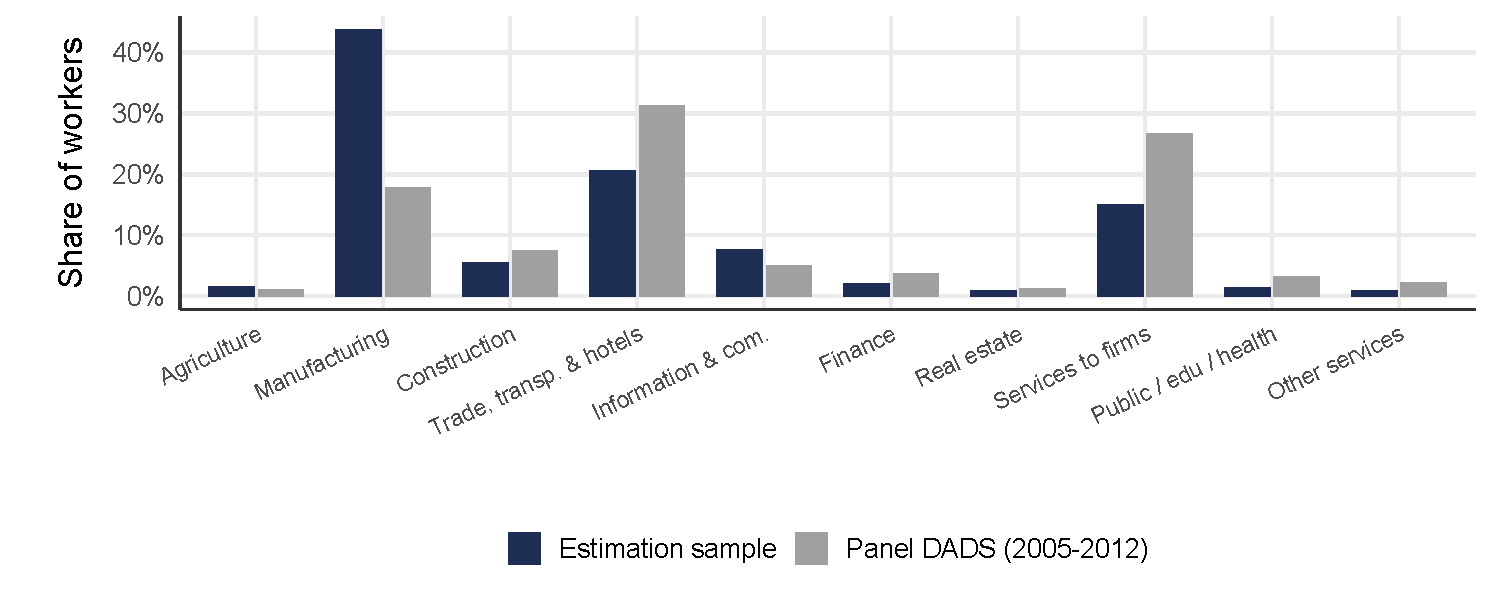
\includegraphics[width=\linewidth, trim={0cm 0cm 0cm 0cm}, clip=true,max width=\linewidth]{figures/02_descriptive_figures/figure_A17_a_mlo_sectors.pdf}
	\end{subfigure}
   
	\begin{subfigure}[b]{\textwidth}
	\caption[]{\small MLO Sample: Occupation\label{fig:desc:MLOocc}}
		\centering
		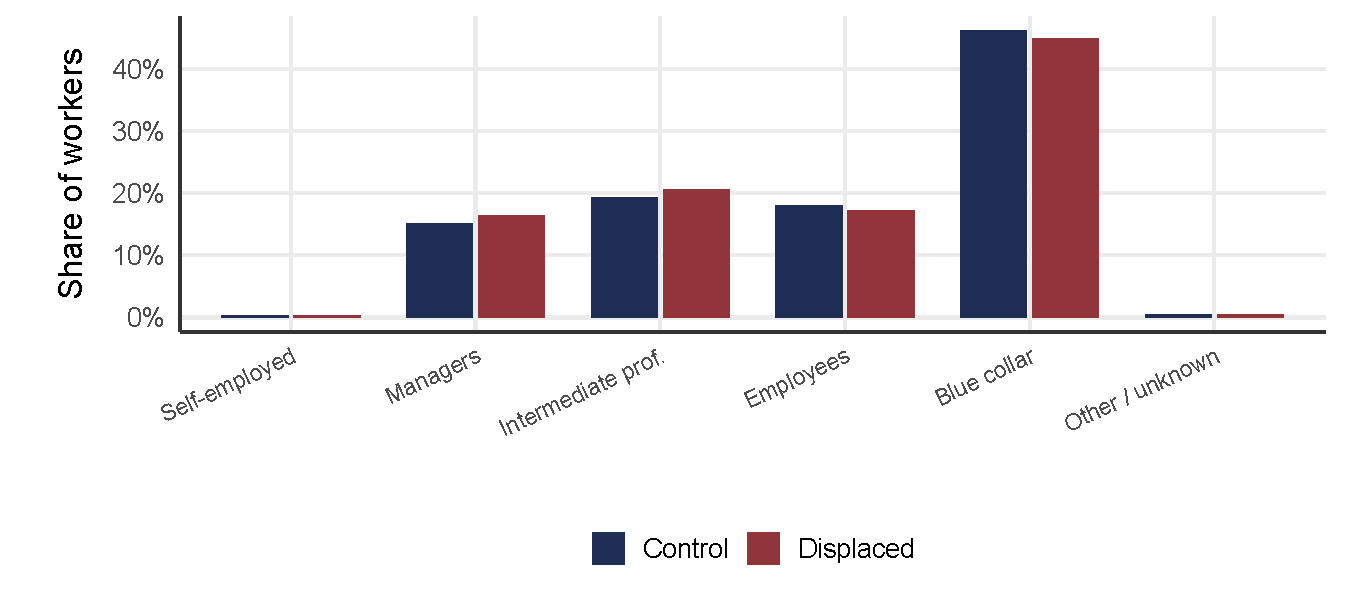
\includegraphics[scale=0.75, trim={0cm 0cm 0cm 0cm}, clip=true,max width=\linewidth]{figures/02_descriptive_figures/figure_A17_b_mlo_occupations.pdf}
	\floatfoot{\footnotesize{\textsc{Notes}: This figure presents descriptive statistics about the sample of 17,949 individuals displaced in a mass layoff (MLO30) and their respective matched controls \textcolor{orange}{[17,946]}. Data is observed at $t^D-1$. Panel (a) reports the distribution of workers across NACE A10 sectors for our \emph{estimation sample} (controls only) and---for reference---the population of private-sector workers in the DADS panel over 2005--2012. We display the control group only because sector is a matching variable, so the MLO-displaced and control-group distributions coincide at $t^D-1$ by construction; controls measured at $t^D-1$ are therefore an accurate description of the sectoral composition of the matched estimation sample. The third bar (Panel DADS) allows the reader to gauge how representative our estimation sample is of the broader French private-sector workforce. Panel (b) displays the distribution of workers across occupations. This variable was not used in the matching algorithm. The sample appears to be balanced across treatment and controls.}}
	\end{subfigure}
\end{figure*}
